\documentclass[border=12pt]{standalone}
\def\pgfsysdriver{pgfsys-dvisvgm.def}
\usepackage[dvisvgm]{xcolor}
\usepackage{xeCJK}
\setCJKmainfont{HaranoAjiGothic-Regular.otf}[BoldFont=HaranoAjiGothic-Bold.otf]
\setCJKsansfont{HaranoAjiGothic-Regular.otf}[BoldFont=HaranoAjiGothic-Bold.otf]
\usepackage{amsmath,amssymb,tikz,lmodern}
\usetikzlibrary{arrows.meta,positioning,calc,fit,backgrounds}
\renewcommand{\familydefault}{\sfdefault}
\definecolor{ink}{HTML}{25322F}
\definecolor{green}{HTML}{246657}
\definecolor{tint}{HTML}{EEF4F0}
\definecolor{soft}{HTML}{C6D2CC}
\definecolor{muted}{HTML}{52615B}
\newif\ifJapanese
\newcommand{\Tx}[2]{\ifJapanese #1\else #2\fi}
\newcommand{\Eff}{\overline{\operatorname{Eff}}}
\newcommand{\heading}[3]{{\color{green}\bfseries #1\quad\Tx{#2}{#3}}\\[5pt]}
% A white rectangle makes the complete citation label clickable, including spaces.
\newcommand{\refurl}[2]{\special{dvisvgm:raw <a xlink:href="#1" target="_blank" rel="noopener noreferrer">}{\setlength{\fboxsep}{0pt}\colorbox{white}{\color{green}\underline{\strut #2}}}\special{dvisvgm:raw </a>}}
\tikzset{
 card/.style={draw=soft,fill=white,rounded corners=2pt,align=left,text=ink,font=\fontsize{10.5}{14}\selectfont,inner xsep=12pt,inner ysep=10pt,text width=14.4cm},
 half/.style={card,text width=6.45cm,minimum height=2.05cm},
 result/.style={card,draw=green,fill=tint,line width=.9pt},
 reason/.style={align=left,text=muted,font=\fontsize{9}{12}\selectfont,inner sep=0pt,text width=12.7cm},
 branchreason/.style={reason,text width=5.95cm},
 edge/.style={-{Stealth[length=2.4mm]},draw=green,line width=1pt},
 wire/.style={draw=green,line width=1pt},
}
% Keep the arrow in a dedicated left gutter; explanations never cover it.
\newcommand{\flow}[3]{
 \coordinate (#2-from) at ($(#1.south)+(-6.9,0)$);
 \coordinate (#2-to) at ($(#2.north)+(-6.9,0)$);
 \draw[edge] (#2-from)--(#2-to);
 \node[reason,anchor=west] (#2-reason) at ($(#2-from)!.5!(#2-to)+(.55,0)$) {#3};
}

\newcommand{\Cite}[2]{\refurl{#1}{#2}}

\Japanesetrue
\begin{document}
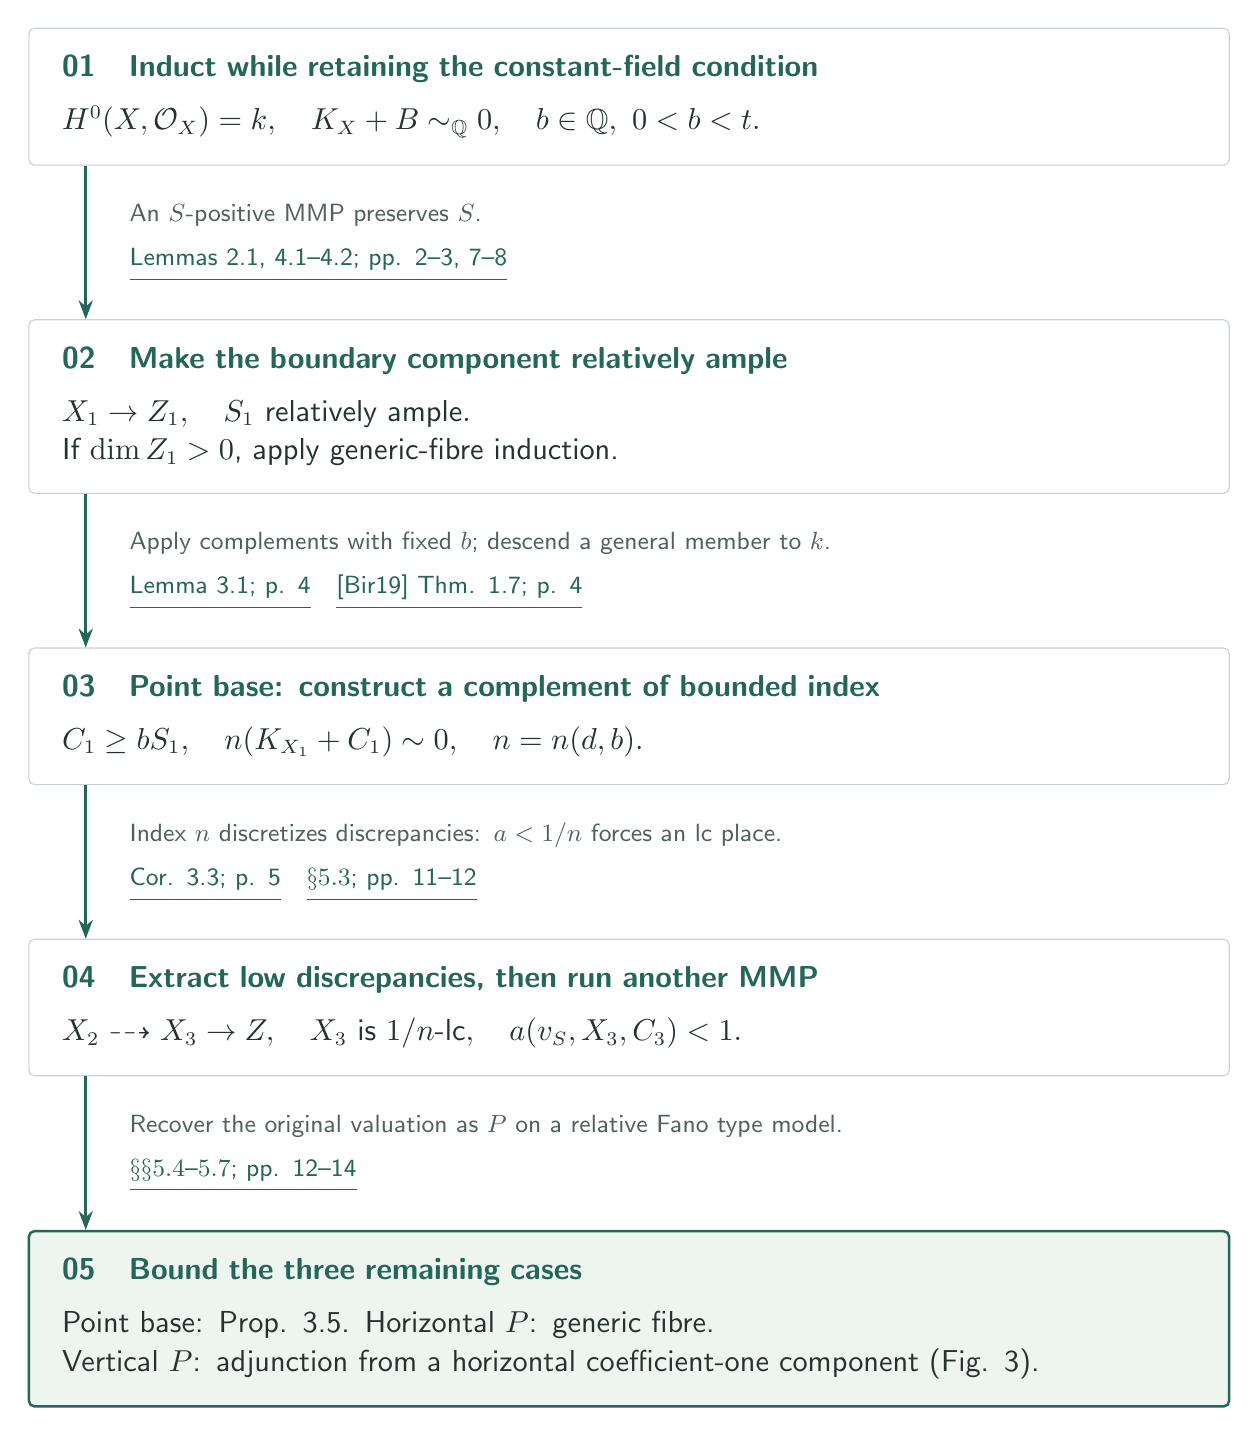
\begin{tikzpicture}
\node[card] (n0) {\heading{01}{定数体を保って次元帰納}{Induct while retaining the constant-field condition}$H^0(X,\mathcal O_X)=k,\quad K_X+B\sim_{\mathbb Q}0,\quad b\in\mathbb Q,\ 0<b<t.$};
\node[card,below=1.95cm of n0] (n1) {\heading{02}{境界成分を相対的に豊富にする}{Make the boundary component relatively ample}$X_1\to Z_1,\quad S_1\text{ relatively ample}.$\\ \Tx{$\dim Z_1>0$：一般ファイバーへ帰納。}{If $\dim Z_1>0$, apply generic-fibre induction.}};
\flow{n0}{n1}{\Tx{負性補題で $S$ を残すMMP。}{An $S$-positive MMP preserves $S$.}\\[4pt]\Cite{https://github.com/openai/math/blob/adc7f1241b42e322a6451854ab7e4b4c146bf78a/preprints/Arithmetic-Stein-degree-bounds-for-log-Calabi-Yau-pairs-September-25-2026/paper.pdf}{Lemmas 2.1, 4.1--4.2; pp. 2--3, 7--8}}
\node[card,below=1.95cm of n1] (n2) {\heading{03}{底が点：有界な指数の補完を作る}{Point base: construct a complement of bounded index}$C_1\ge bS_1,\quad n(K_{X_1}+C_1)\sim0,\quad n=n(d,b).$};
\flow{n1}{n2}{\Tx{固定係数 $b$ に補完を適用し、一般元で $k$ へ降下。}{Apply complements with fixed $b$; descend a general member to $k$.}\\[4pt]\Cite{https://github.com/openai/math/blob/adc7f1241b42e322a6451854ab7e4b4c146bf78a/preprints/Arithmetic-Stein-degree-bounds-for-log-Calabi-Yau-pairs-September-25-2026/paper.pdf}{Lemma 3.1; p. 4}\quad \Cite{https://arxiv.org/pdf/1603.05765v4}{[Bir19] Thm. 1.7; p. 4}}
\node[card,below=1.95cm of n2] (n3) {\heading{04}{低discrepancyを抽出し、再びMMP}{Extract low discrepancies, then run another MMP}$X_2\dashrightarrow X_3\to Z,\quad X_3\text{ is }1/n\text{-lc},\quad a(v_S,X_3,C_3)<1.$};
\flow{n2}{n3}{\Tx{指数 $n$ がdiscrepancyを離散化：$a<1/n$ なら補完のlc place。}{Index $n$ discretizes discrepancies: $a<1/n$ forces an lc place.}\\[4pt]\Cite{https://github.com/openai/math/blob/adc7f1241b42e322a6451854ab7e4b4c146bf78a/preprints/Arithmetic-Stein-degree-bounds-for-log-Calabi-Yau-pairs-September-25-2026/paper.pdf}{Cor. 3.3; p. 5}\quad \Cite{https://github.com/openai/math/blob/adc7f1241b42e322a6451854ab7e4b4c146bf78a/preprints/Arithmetic-Stein-degree-bounds-for-log-Calabi-Yau-pairs-September-25-2026/paper.pdf}{$\S5.3$; pp. 11--12}}
\node[result,below=1.95cm of n3] (n4) {\heading{05}{残る三場合をそれぞれ抑える}{Bound the three remaining cases}\Tx{点の底：Prop. 3.5。水平な $P$：一般ファイバー。\\垂直な $P$：水平係数1成分から随伴（第3図）。}{Point base: Prop. 3.5. Horizontal $P$: generic fibre.\\Vertical $P$: adjunction from a horizontal coefficient-one component (Fig. 3).}};
\flow{n3}{n4}{\Tx{元の付値を相対Fano typeモデル上の $P$ として回復。}{Recover the original valuation as $P$ on a relative Fano type model.}\\[4pt]\Cite{https://github.com/openai/math/blob/adc7f1241b42e322a6451854ab7e4b4c146bf78a/preprints/Arithmetic-Stein-degree-bounds-for-log-Calabi-Yau-pairs-September-25-2026/paper.pdf}{$\S\S5.4$--$5.7$; pp. 12--14}}
\end{tikzpicture}

\end{document}
